%!TEX root = ../../../main.tex
\section{Navigation Controller} % (fold)
\label{sec:mr_navigation_controller}
Using the processed information from the sensors and the different kind of navigations, the robot is able to move and satisfy all the requirements from the project.
In this section the \emph{navigation controller} is explained.
This is in charge of finding the path, and actions associated to said path, given two nodes.

\subsection{Navigation state representation} % (fold)
    \label{sub:mr_navigation_state_representation}
    In order to navigate from one position to the desired one, a graph of the possible states in which the robot is stopped or idle has been represented.
    This graph depicts all the possible states of the mobile robot in which the robot has not movement along with their associated transference functions. 
    These are other states in which the robot is moving or changing its state and that in this project will be referred as \emph{skills} (Section \ref{sub:skills}).
    In the figure \ref{fig:mr_graph} the graph of the project is shown.
    
    \begin{figure}[H]
        \centering
        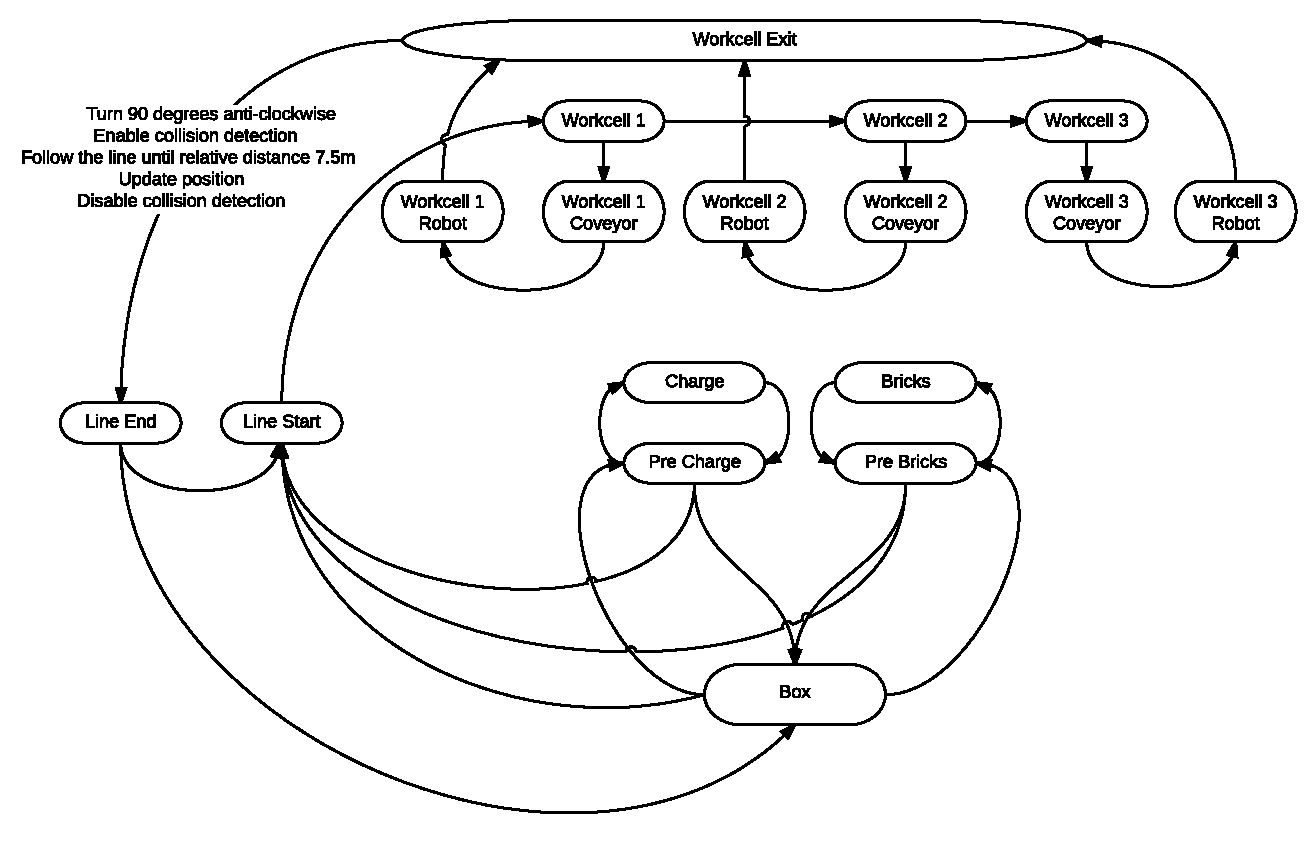
\includegraphics[width=\textwidth]{figs/mr_graph.pdf}
        \caption{Graph representation adopted in the project}
        \label{fig:mr_graph}
    \end{figure}

    As an example, in the transference between the node \emph{"Workcell Exit"} and \emph{"Line End"}, the associated conditions are shown. 
    These are: first, needs to \emph{turn 90 degrees clockwise}, then \emph{follow the line until the QR "line\_end"} is detected, all this done with the collision detector turned on and changing the internal position of the robot in the end.
    % subsection navigation_state_representation (end)

    \subsection{Skills} % (fold)
    \label{sub:skills}
    As stated before, the skills are available actions to transfer the robot from one navigation state to another. They let the robot change its state and position.
    The implementation is based on a couple between one of the navigation types and some information from the sensors used as a condition.
    The skills designed and implemented are:
    \begin{itemize}
        \item Follow the line until desired QR
        \item Follow the line until desired LIDAR distance
        \item Follow the line until desired relative distance
        \item Linear relative move
        \item Angular relative move
        \item Go to free position
        \item Detect obstacles
        \item Wait
        \item Specialized charging skill
        \item Initialising the AMCL 
    \end{itemize}    
	An example of the skills associated with the transition from one node to another is shown in figure \ref{fig:mr_graph}. The skill list shown only facilitate the transfer when exiting from work-cell 1, due to the use of the follow line until relative distance. This distance will be different for each work-cell.

The navigation skills have previously been described. The specialized charging skill combines multiple of the other skills. Initially the robot moves to a position in free space. Then it follows a line until a certain LIDAR distance. Here it waits 10 seconds to see if the battery level has risen. If it has risen the state is set to charge. Otherwise the robot reverses and restarts the process. \\
The last skill, initialising the AMCL, is used when the robot transitions from the line navigation to free navigation. This is necessary because the AMCL looses its position when the robot moved into the robot cells.
	
	
    % subsection skills (end)

    \subsection{Graph search} % (fold)
    \label{sub:mr_graph_search}
    In order to find the most optimal path between two nodes in the graph a graph search algorithm has been implemented.
    All the transfers between states have an associated cost which is used by a Breadth First Search (BFS).

    The BFS is an algorithm of searching in graphs that explores all the neighbours of the root, then the neighbours of this ones etc.
    BFS is a complete search algorithm and optimal meaning that will always find the optimal solution.
    In this case as the cost between nodes is a given distance, the BFS will always find the shortest path.
    
    The negative part of the BFS is the space complexity but due to the graph being rather small, the search time is in the order of milliseconds.
    % subsection artificial_intelligence (end)
% section navigation_controller (end)
